%%%%%%%%%%%%%%%%%%%%%%%%%%%%%%%%%%%%%%%%%%%%%%%%%%%%%%%%%%%%%%%%%%%%%%%%%%%%%%%%
%2345678901234567890123456789012345678901234567890123456789012345678901234567890
%        1         2         3         4         5         6         7         8

\documentclass[letterpaper, 10 pt, conference]{ieeeconf}  % Comment this line out
                                                          % if you need a4paper
%\documentclass[a4paper, 10pt, conference]{ieeeconf}      % Use this line for a4
                                                          % paper

\IEEEoverridecommandlockouts                              % This command is only
                                                          % needed if you want to
                                                          % use the \thanks command
\overrideIEEEmargins
% See the \addtolength command later in the file to balance the column lengths
% on the last page of the document

\usepackage[utf8]{inputenc}
\usepackage[T1]{fontenc}
\usepackage[makeroom]{cancel}
\pagenumbering{roman}
\usepackage{graphicx}
\usepackage{multirow}
\usepackage{physics}
\usepackage{amsmath}
\newcommand{\nwsearrow}{%
  \mathrel{\text{\ooalign{$\nwarrow$\cr$\searrow$}}}%
}
\newcommand{\neswarrow}{%
  \mathrel{\text{\ooalign{$\swarrow$\cr$\nearrow$}}}%
}
\usepackage{amssymb}
\usepackage{cite}
% The following packages can be found on http:\\www.ctan.org
%\usepackage{graphics} % for pdf, bitmapped graphics files
%\usepackage{epsfig} % for postscript graphics files
%\usepackage{mathptmx} % assumes new font selection scheme installed
%\usepackage{mathptmx} % assumes new font selection scheme installed
%\usepackage{amsmath} % assumes amsmath package installed
%\usepackage{amssymb}  % assumes amsmath package installed

\title{\LARGE \bf
Integrated silicon photonics as a platform for quantum cryptographic tasks
}

%\author{ \parbox{3 in}{\centering Huibert Kwakernaak*
%         \thanks{*Use the $\backslash$thanks command to put information here}\\
%         Faculty of Electrical Engineering, Mathematics and Computer Science\\
%         University of Twente\\
%         7500 AE Enschede, The Netherlands\\
%         {\tt\small h.kwakernaak@autsubmit.com}}
%         \hspace*{ 0.5 in}
%         \parbox{3 in}{ \centering Pradeep Misra**
%         \thanks{**The footnote marks may be inserted manually}\\
%        Department of Electrical Engineering \\
%         Wright State University\\
%         Dayton, OH 45435, USA\\
%         {\tt\small pmisra@cs.wright.edu}}
%}

\author{Daniel Hutama$^{1}$ and Adrian Chan$^{1}$% <-this % stops a space
\thanks{$^{1}$The Photonic Systems Group, Department of Electrical and Computer Engineering, McGill University, 3480 University St. room 753, Montreal, Quebec H3A 2A7}
}


\begin{document}



\maketitle
\thispagestyle{empty}
\pagestyle{empty}


%%%%%%%%%%%%%%%%%%%%%%%%%%%%%%%%%%%%%%%%%%%%%%%%%%%%%%%%%%%%%%%%%%%%%%%%%%%%%%%%
\begin{abstract}


Contemporary classical cryptographic protocols exhibit vulnerabilities to attacks from emerging quantum technologies. Most notably, a quantum device capable of performing Shor's algorithm can efficiently defeat the commonly used RSA asymmetric key distribution protocol. Here, we describe how integrated silicon photonics provides a platform for such a quantum device. In addition, we discuss how silicon photonics can provide a provably secure alternative to vulnerable communication protocols by facilitating scalable quantum key distribution (QKD). In particular, we discuss an implementation of the BB84 QKD protocol in integrated silicon photonics. The goal of this paper is to highlight how silicon photonics provides a platform to both attack and resolve weaknesses in classical information security. 

\end{abstract}


%%%%%%%%%%%%%%%%%%%%%%%%%%%%%%%%%%%%%%%%%%%%%%%%%%%%%%%%%%%%%%%%%%%%%%%%%%%%%%%%
\section{Introduction}


Integer factorization is a problem that has been studied by mathematicians for centuries, but has yet to see an efficient classical solution. The apparent intractability of the factorization problem has become the cornerstone of several cryptosystems, such as the widely used RSA encryption scheme \cite{RSA78}. Several modern internet security protocols, such as Secure Shell, SSL/TLS, S/MIME, and OpenPGP, rely on RSA encryption, making RSA one of the most economically important cryptographic systems. 

At its core, the RSA scheme is an asymmetric encryption protocol, in which a message's receiver generates a public key/private key pair. The recipient then
broadcasts the public key and safeguards the private key. Any sender can use the broadcasted public key to encrypt a message, while only the receiver can decrypt messages using the private key. The primary vulnerability in the RSA scheme lies in the public key, which obfuscates the private key behind the integer factorization problem. If integer factorization can be performed efficiently, the private key can be obtained from the public key and used to decrypt any past and future messages encrypted with the public key.

In 1994, Peter Shor published a quantum algorithm capable of factoring an $n$-bit integer $N$ in a number of steps polynomial in the input size (i.e. the bit-length $n$) \cite{shor94}. In particular, Shor's algorithm factors an $n$-bit integer with a time complexity of $\mathcal{O}(n^2(\log n)(\log(\log n)))$, while the most efficient known classical factoring algorithm runs with a time complexity of $\mathcal{O}(\exp((\frac{64}{9})^{1/3} n^{1/3}(\log n)^{2/3})$ \cite{GNFS}. The realization of a quantum computer running Shor's algorithm (with a sufficient number of qubits capable of maintaining quantum coherence and performing error correction) may one day make the large-N factorization problem tractable, thus breaking the effectiveness of RSA. 

In this paper, we discuss recent developments in silicon photonics related to modern encryption. We first discuss how silicon photonics provides a platform to attack RSA encryption via an implementation of Shor's algorithm. Following this, we discuss how silicon photonics facilitates a quantum-secure encryption alternative. Specifically, we discuss a recent implementation of the BB84 quantum key distribution (QKD) protocol, which is used to establish symmetric (shared) private keys between the sender and receiver for use in unbreakable one-time pads. 

\section{Shor's Algorithm}
Instead of utilizing a brute-force approach, Shor's algorithm considers a related number-theoretic problem. In particular, Shor's approach is to compute $r$, the period of $a$ modulo $N$, where $a$ is a randomly chosen seed value between $1$ and $N$. The factorization of $N$ can be accomplished via period-finding in five (high level) steps: (1) Pick a random seed value $a$, with $1 < a < N$. (2) Compute the greatest common divisor of $a$ and $N$ via the Euclidean algorithm. If $\gcd(a,N) \not = 1$, we have found a non-trivial factor of $N$. If $\gcd(a,N)=1$, continue. (3) Compute $r$, the period of $a \pmod{N}$, i.e. find $r$, such that $a^r \equiv 1 \pmod{N}$. (4) Check that $r$ is even and that $a^{r/2}\not \equiv \pm 1 \pmod{N}$. If this condition is violated, return to step 1. Otherwise, continue. (5) The factorization of $N = pq$ is achieved by computing $p = \gcd(a^{r/2} - 1, N)$ and $q = \gcd(a^{r/2} + 1, N)$ \cite{shor94}.

The focus of Shor's algorithm is on step (3), which is made efficient on a quantum computer \cite{shor94, shorssmall}. In short, Shor's algorithm begins with a quantum computer initialized with two entangled quantum registers. The qubits in the first register are placed in a superposition state using Hadamard gates. Following this, modular exponentiation is applied on the second register, conditional on the states of the qubits in the first register. A Fourier transform is applied to the first register to encode the function's period in a measurement probability amplitude. Finally a measurement of the first register yields classical data, from which we can obtain the function's period using the classical method of continued fractions \cite{shor94}.


\subsection{Silicon Photonics}

While Shor's algorithm is proven to be able to factor an integer exponentially faster than classical algorithms, it has yet to be implemented on a scale large enough to be a threat to modern encryption. The most efficient known quantum circuit description of Shor's algorithm for an arbitrary integer of bit-size $n$ requires a quantum circuit of size $2n + 2$ qubits \cite{shorssmall}. At time of writing, the most powerful universal quantum computers can manipulate up to $54$ qubits, much less than is required to break 1024-bit RSA \cite{googlequbit}. However, compiled versions (i.e. one in which the factors are already known) of Shor's algorithm have been demonstrated in experiments with liquid-state NMR and bulk optical logic gates \cite{logicgate}. Such compiled versions can operate with fewer than the $2n+2$ qubits required for arbitrary integer factorization. 
%As we will discuss, newer implementations have been demonstrated in silicon photonics, which provides a more compact platform with the additional advantage of manufacturing scalability. 

Politi \textit{et al.} demonstrate a compiled device that is able to factor $N = 15$ $(n=4)$ into its prime factors, $p=3$ and $q=5$, using five photonic qubits. In their compiled version, they choose $a = 2$. This specific choice of compilation reduces the total number of qubits needed, and also eliminates the need to impliment a quantum Fourier transform \cite{Shorphotonics}. 

The fabricated device is a silicon photonic circuit in which four primary single photons and one auxiliary photon are generated via spontaneous parametric down-conversion (SPDC) and simultaneously injected into the circuit via edge-coupling. The primary photons are initialized in the path state $\ket{0}_{x1}\ket{0}_{x2}\ket{0}_{f1}\ket{1}_{f2}$ where the bit value is determined by the input port, as shown in Figure \ref{fig:1}b. Qubits are then placed in a superposition of all possible four-bit states via Hadamard gates, which are implemented with half-reflectivity directional couplers. The compiled function is then implemented with two independent, non-deterministic controlled phase (CZ) gates, which are formed by a network of three 1/3 directional couplers. In particular, the function imparts a controlled phase shift on the qubit in the $f_i$ register, dependent on the corresponding qubit in the $x_i$ register being in the $\ket{1}$ state. 

As a result of the quantum nature of the single photons passing through the circuit, the output of the device is probabilistic and determined by the specific photon path on each trial. Results in Figure \ref{fig:1}c, show the measurement results of the first ($x_i$) register, where the four binary outcomes are $000_2$, $010_2$, $100_2$, and $110_2$, corresponding to the decimal values of 0, 2, 4, and 6, respectively. The first result, $000_2$, is an expected failure inherent to Shor's algorithm. The third result $100_2$ yields trivial factors $1$ and $15$, while the second and fourth results yield $r=4$ via the method of continued fractions \cite{Shorphotonics}. The expected results of $p=\gcd(2^{4/2}-1,15) = 3$ and $q=\gcd(2^{4/2}+1, 15) = 5$ can then be classically computed via the Euclidean algorithm. 

While Shor's algorithm in silicon photonics has been limited to compiled versions, such experiments show the potential it has in the field of quantum computing. As the field evolves with other quantum technologies, it will become increasingly important to develop encryption protocols that are resistant to quantum attacks. We show in the next section how silicon photonics is uniquely positioned to facilitate the widespread adoption of a quantum secure protocol. 

\begin{figure}[htbp]
    \centering
    \includegraphics[width = 0.485\textwidth]{"Shor_circuit".PNG}
    \caption{\textbf{a}, Quantum circuit. \textbf{b}, Schematic of waveguide on the chip device. Qubits in the first register are denoted $x_i$, while qubits in the second register are denoted $f_i$. \textbf{c}, Results of measurement on the first register after applying the function. \cite{Politi}}
    \label{fig:1}
\end{figure} 

\section{Quantum Key Distribution}
Silicon photonics is a promising platform for quantum key distribution (QKD), since bit states can easily be encoded in several different ways. For instance, binary 1s and 0s can be implemented via photon path, polarization, or incident power to name a few. Furthermore, by utilizing the widely available and mature CMOS fabrication technologies, silicon photonics can facilitate the widespread distribution of quantum communication devices. In this section, we discuss an implementation of QKD in silicon photonics. Following this, we discuss recent developments regarding single photon generation and detection in silicon photonics for use in quantum information technologies.


\subsection{BB84} The BB84 QKD protocol is a provably secure, symmetric key distribution protocol \cite{bb84paper,bb84security}. In the BB84 scheme, two parties, Alice and Bob, wish to establish a shared private key to securely encrypt subsequent transmissions. To establish the shared key, Alice transmits a sequence of bits, which are randomly prepared in one of two polarization bases. For instance, we can define the $+$ basis in which binary $\ket{1_+}$ corresponds to vertical polarization $\ket{\updownarrow}$ and binary $\ket{0_+}$ corresponds to horizontal polarization $\ket{\leftrightarrow}$. In the $\times$ basis, binary $\ket{1_\times}$ corresponds to $135^\circ$ polarization $\ket{\nwsearrow}$, while binary $\ket{0_{\times}}$ corresponds to $45^\circ$ polarization $\ket{\neswarrow}$. Bob then measures the received bit in one of the two polarization bases. If the measurement basis matches the generation basis, Bob will measure the correct bit value (e.g. $||\braket{1_+}{1_+}||^2 =1$, $||\braket{0_+}{1_+}||^2=0$). However, if the measurement basis is incorrect, Bob will measure the correct bit with 50\% probability (e.g. $||\braket{1_\times}{1_+}||^2 = ||\braket{0_\times}{1_+}||^2= 0.5$). Once Bob publicly announces that he has received Alice's transmission, Alice communicates her choice of bases to Bob. Both Alice and Bob discard the bits in which the bases do not match. The remaining bits form the shared secret key. 

The security of the protocol comes from the no-cloning theorem, which prevents an eavesdropper, Eve, from covertly tapping the channel without disturbing the states of Alice's transmitted bits \cite{bb84security}. If Eve were to attempt to intercept and re-transmit the secret key, her measurements would collapse the states of the bits transmitted by Alice. The discrepancy can then be detected statistically during the resolution phase between Alice and Bob. If this discrepancy is detected, Alice and Bob can simply restart the protocol.

\subsection{BB84 in Silicon Photonics.}

Bunandar \textit{et al.} demonstrate a QKD encoder in silicon photonics based on the BB84 protocol \cite{metroQKD}. The device consists of a 10 Gbps Mach-Zehnder modulator (MZM) with polarization-splitting grating couplers (PSGCs), shown in Figure \ref{fig:pathencoding}. The PSGCs are used to convert the orthogonal components of the elliptically polarized field in the input fiber into separate TE mode paths on the PIC and vice-versa \cite{PSGC}. Within the PIC, the relative phases between the two paths are controlled using the MZM. The phase modulators are based on depletion-mode free-carrier dispersion implemented with a doped $p$-$i$-$n$ junction. The overlap of the free-carriers and optical mode results in free-carrier refraction. Phase modulation is achieved by controlling the refraction via gigahertz RF signals. The photon polarization in the output fiber is controlled by the relative phase shift between the top and bottom paths imparted by the MZM.

\begin{figure}[!ht]
    \centering
    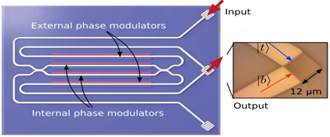
\includegraphics[width = 0.485\textwidth]{pathencoding.PNG}
    \caption{From \cite{metroQKD}. Silicon photonic path-to-polarization encoder for the BB84 protocol.}
    \label{fig:pathencoding}
\end{figure} 

The device is initialized to produce the state $(\ket{t} + \ket{b})/\sqrt{2}$, which is set as the $\ket{0_+}$ state. The MZM is then adjusted to generate $(\ket{t} + e^{i\phi}\ket{b})/\sqrt{2}$, where $\phi$ is the phase shift applied by using RF signals of differing voltages. All four required states for the BB84 protocol can be generated by applying phase shifts of $\phi = 0, \pi/2, \pi$, and $3\pi/2$, as shown in Table \ref{tab:tab1}. Following transmission over a 43 km fiber, the polarization states are measured using a polarization beam splitter followed by InGaAs photodiodes. At 10 Gbps, the BER is measured at $9.0 \cdot 10^{-10} s^{-1}$.



\begin{table}[!ht]
\caption{Correspondence between path states and BB84 states.}
\label{tab:tab1}
\centering
\begin{tabular}{|c|c|c|c|}
\hline
\textbf{$\phi$} & \textbf{Path State} & \textbf{Defined Pol. State} & \textbf{Defined Bit State} \\ \hline
$0$ & $\dfrac{\ket{t} + \ket{b}}{\sqrt{2}}$ & $\ket{\leftrightarrow}$ & $\ket{0_+}$ \\ \hline
$\pi$ & $\dfrac{\ket{t} - \ket{b}}{\sqrt{2}}$ & $\ket{\updownarrow}$ & $\ket{1_+}$ \\ \hline
$\pi/2$ & $\dfrac{\ket{t} + i\ket{b}}{\sqrt{2}}$ & $\ket{\neswarrow}$ & $\ket{0_\times}$ \\ \hline
$3\pi/2$ & $\dfrac{\ket{t} - i\ket{b}}{\sqrt{2}}$ & $\ket{\nwsearrow}$ & $\ket{1_\times}$ \\ \hline
\end{tabular}
\end{table}

\pagebreak

\subsection{Single Photon Generation}
The technologies mentioned above all use SPDC in order to inject single photons into their photonic device. This method leads to significant losses in performance due to mechanisms such as coupling loss. In order to overcome this, much focus has gone into integrated sources, which removes the need to couple light into their photonic circuit. One common method for the generation of single photons is through spontaneous four-wave mixing (SFWM). SFWM can be realized through the mixing of two or three wavelengths to produce one or two new wavelengths. This process requires the energy to be conserved and is extremely phase sensitive. Therefore, PICs, which are phase-stable, are a good candidate to realize this process. Although it is possible to produce single photons through SFWM, efficiencies are diminished from spectral purity caused from background noise of surrounding components. 

In order to overcome the weaknesses of SFWM, an improved design has been adopted by researchers - micro-ring resonators (MRRs) with SFWM \cite{SPS}. By utilizing MRRs, single-photon generation with high spectral purity and without any filters is possible. This results in higher efficiencies compared to the conventional SFWMs method. Furthermore, by implementing MRRs and SFWMs synergistically, noise can be minimized through a weak optical pump. With only one additional component in the PIC design, the single photon source (SPS) can be simplified and enhanced for scalable applications.

One example of using a MMR with SFWM device is demonstrated by Llewellyn \textit{et al.} \cite{SPS}. Here, they design and experimentally test a four-photon, four-qubit MRR with SFWM-based single photon generator. By utilizing four identical MRRs within their design, they are able to generate pure and indistinguishable photons with high efficiency while minimizing the background noise from the surrounding components within the circuit. While background noise is minimized by the MRRs, the photons are indistinguishable due to interference created by the Mach Zehnder interferometers (MZIs) within the circuit \cite{SPS}. In the transmitter circuit, two pairs of non-degenerate photons are generated in the array of MRR SPSs. The four photons are demultiplexed by asymmetric MZIs and routed via waveguide crossings. Utilizing thermal-optic phase shifters on the MZIs allows for the projective measurements of the multi-qubit states. In the receiver circuit, the polarization-encoded qubits are converted to path encoding and then measured by an external avalanche photodetector.

% \begin{figure}[!ht]
%     \centering
%     \includegraphics[width = 0.5\textwidth]{"MRR_SPS".PNG}
%     \caption{\textbf{a}, Multi-qubit entanglement transmitter circuit based on a MMR with SFWM system. \textbf{b}, The receiver circuit which is linked to the transmitter by a 10 m single-mode fibre. \textbf{c}, SEM image of the MRR SPS design coupled to a bus waveguide. \textbf{d}, SEM image of the subwavelength grating coupler. Top: 1D subwavelength grating coupler for fibre-chip interface. Bottom: 2D subwavelength grating coupler for path-polarization conversion.}
%     \label{fig:2}
% \end{figure}

The group experimentally demonstrated signal and idler photons at 1539.758 nm and 1559.015 nm, indicating an ability to achieve single photon generation in the region where silicon has the lowest attenuation. SFWM gain was also measured and background noise was found to be suppressed due to the advantage of having MRRs. Spectral indistinguishability, another parameter of interest, was measured and determined to have a visibility of 90.99 $\pm$ 3.91\%. Lastly, quantum interference between pairwise MMRs was found to be excellent with an average of 87.3 $\pm$ 1.9\% with multi-pair correction. These results provide a usable and simple design that demonstrates how silicon photonics can be used and scaled for quantum information applications.


\subsection{Single Photon Detection}
Many tasks in quantum communications are dependent on single-photon qubits. Due to the very small energies ($\sim 10^{-19}$ J) involved, single photon detectors (SPDs) must be used. Some popular examples of SPDs include avalanche photodiodes, superconducting nanowire single-photon detectors (SNSPDs), and transition edge sensors \cite{bulkoptics}. 

One current issue that researchers are attempting to solve is that SPDs can only achieve high efficiencies as an external stand-alone device. Having an external stand-alone device leads to additional losses such as from fibre coupling and material absorption outside the detector \cite{SNSPD}. SNSPDs allow for an integrated SPD which provides a unique advantage compared with external devices, as it prevents additional insertion loss mechanisms. Furthermore, SNSPDs have been found to offer high internal quantum efficiencies and low-timing jitter at liquid helium temperature, whereas current alternatives must operate at even colder temperatures in the millikelvin range. Lastly, most integrated devices are compatible with current CMOS fabrication techniques, allowing for easy scalability. 

% SNSPD's are able to convert single photons into electrical current by operating below the superconducting critical temperature and biased with a DC current close to the superconducting critical current. When a photon is of normal incident on the nanowire, the energy is absorbed and pairs of electrons are broken which creates a localized non-superconducting region. This region creates a shunt to the amplifier which results in a measurable voltage. The region then returns back to its superconducting state when it is cooled.

One example of an integrated single-photon detector is demonstrated by Pernice \textit{et al.} \cite{SNSPD}. Here, they fabricated and demonstrated a highly efficient and repeatable integrated SPD device at telecom wavelengths. Single photons are first generated externally and coupled into the device, then split at a 50/50 splitter. One path leads to the SNSPD and the other path leads to a control port for baselining, as shown in Figure 3. Remaining light that was not collected by the detector is collected at the residual light port. From their results, they were able to obtain a on-chip single-photon detection efficiency of 91\%, dark count rate of 5886 Hz, and a timing jitter of 18 ps. This device presented not only high detection efficiency, but also extremely fast timing jitter, which represents the time it takes for a photon to be absorbed by the detector and converted into electrical signal. Although the dark count rate was found to be high, the researchers noted that the detection rate was within the MHz range, and that dark counts within the kHz range had negligible affect on the detection efficiency. SNSPD designs are constantly being improved, such as the addition of low-loss delay lines to create photon buffering, resulting in increased quantum efficiencies and speed. However, one crucial limitation still remains for the SPD field, which requires extremely low temperature operations to detect single-photons.

\begin{figure}[htbp]
    \centering
    \includegraphics[width = 0.485\textwidth]{"SNSPD".PNG}
    \caption{\textbf{a}, SNSPD structure. \textbf{b}, Optical micrograph of integrated circuit.}
    \label{fig:3}
\end{figure} 
% Parameters to investigate to quantify the performance of SPDs include spectral range, dead time, dark count rate, detection efficiency, timing jitter, and ability to resolve photon number. 




\section{Conclusion}

While there is still room for improvement in device power and efficiency, silicon photonics provides a platform for tremendously powerful and compact quantum computation devices. As the field continues to evolve, it is likely that devices capable of manipulating a greater number of qubits will emerge. As such devices pose a threat to modern communication security, it is essential to develop quantum-secure alternatives to contemporary quantum-susceptible protocols. 

Fortunately, silicon photonics also provides a platform for compact and scalable secure communications techologies. Heterogeneous bonding of active laser materials onto silicon PICs can enable fully integrated QKD transmitters. In addition, the integration of single photon generators and detectors necessary for more advanced tasks in quantum information science can accelerate research and commercialization in the field. These integrated devices will be able to leverage the existing manufacturing processes to achieve the widespread adoption of quantum-secure communications protocols.

% \begin{table}[]
% \centering
% \begin{tabular}{|c|c|c|c|c|}
% \hline
% \textbf{$\phi$} & \textbf{Path State} & \textbf{Defined Polarization State} & \textbf{Defined Bit State} & \textbf{BB84 Basis} \\ \hline
% $0$ & $\dfrac{\ket{t} + |b\ket}{\sqrt{2}}$ & $|↔\ket$ & $|0_+\ket$ & \multirow{2}{*}{$+$} \\ \cline{1-4}
% $\pi$ & $\dfrac{|t\ket - |b\ket}{\sqrt{2}}$ & $|↕\ket$ & $|1_+\ket$ &  \\ \hline
% $\pi/2$ & $\dfrac{|t\ket + i|b\ket}{\sqrt{2}}$ & $|⤢\ket$ & $|0_\times\ket$ & \multirow{2}{*}{$\times$} \\ \cline{1-4}
% $3\pi/2$ & $\dfrac{|t\ket - i|b\ket}{\sqrt{2}}$ & $|⤡\ket$ & $1_\times\ket$ &  \\ \hline
% \end{tabular}
% \end{table}

% \section{Silicon Photonics}
% Silicon photonics is a unique and advantageous technology for the field of quantum communication. This is because photons can be manipulated in linear optics to act as a quantum logic gate with no light-matter interactions. This is can be accomplished through the generation, transmission, and detection of single photons which act as states, one and zero, based on their polarization. Furthermore, by utilizing the widely available and mature CMOS fabrication technologies, silicon photonics can be easily scalable for quantum communication applications. 

% Silicon-based photonic integrated circuits (PICs) can be implemented as a more reliable and compact device compared to the traditional fiber-based devices for quantum key distribution (QKD) applications. One main advantage of PICs over fiber-based devices is the stability of the phase and reduced polarization drift. This is because PICs are able to correct the drift in the channel unlike fiber-based devices which require additional components such as narrow filters, spatial filtering, and adaptive optics. 

% \subsection{Single Photon Generation}



% \subsection{Modulation}
% Modulation of qubits is essential process in the achieve quantum communication. Modulation facilitates the change of polarization in a qubit which results different bit states.  


% \subsection{Maintaining the Integrity of the Specifications}

% The template is used to format your paper and style the text. All margins, column widths, line spaces, and text fonts are prescribed; please do not alter them. You may note peculiarities. For example, the head margin in this template measures proportionately more than is customary. This measurement and others are deliberate, using specifications that anticipate your paper as one part of the entire proceedings, and not as an independent document. Please do not revise any of the current designations

% \section{MATH}

% Before you begin to format your paper, first write and save the content as a separate text file. Keep your text and graphic files separate until after the text has been formatted and styled. Do not use hard tabs, and limit use of hard returns to only one return at the end of a paragraph. Do not add any kind of pagination anywhere in the paper. Do not number text heads-the template will do that for you.

% Finally, complete content and organizational editing before formatting. Please take note of the following items when proofreading spelling and grammar:

% \subsection{Abbreviations and Acronyms} Define abbreviations and acronyms the first time they are used in the text, even after they have been defined in the abstract. Abbreviations such as IEEE, SI, MKS, CGS, sc, dc, and rms do not have to be defined. Do not use abbreviations in the title or heads unless they are unavoidable.

% \subsection{Units}

% \begin{itemize}

% \item Use either SI (MKS) or CGS as primary units. (SI units are encouraged.) English units may be used as secondary units (in parentheses). An exception would be the use of English units as identifiers in trade, such as ``3.5-inch disk drive''.
% \item Avoid combining SI and CGS units, such as current in amperes and magnetic field in oersteds. This often leads to confusion because equations do not balance dimensionally. If you must use mixed units, clearly state the units for each quantity that you use in an equation.
% \item Do not mix complete spellings and abbreviations of units: ``Wb/m2'' or ``webers per square meter'', not ``webers/m2''.  Spell out units when they appear in text: ``\ldots a few henries'', not ``\ldots a few H''.
% \item Use a zero before decimal points: ``0.25'', not ``.25''. Use ``cm$^3$'', not ``cc''. (bullet list)

% \end{itemize}


% \subsection{Equations}

% The equations are an exception to the prescribed specifications of this template. You will need to determine whether or not your equation should be typed using either the Times New Roman or the Symbol font (please no other font). To create multileveled equations, it may be necessary to treat the equation as a graphic and insert it into the text after your paper is styled. Number equations consecutively. Equation numbers, within parentheses, are to position flush right, as in (1), using a right tab stop. To make your equations more compact, you may use the solidus ( / ), the exp function, or appropriate exponents. Italicize Roman symbols for quantities and variables, but not Greek symbols. Use a long dash rather than a hyphen for a minus sign. Punctuate equations with commas or periods when they are part of a sentence, as in
% \begin{equation}
% \alpha + \beta = \chi
% \end{equation}

% Note that the equation is centered using a center tab stop. Be sure that the symbols in your equation have been defined before or immediately following the equation. Use ``(1)'', not ``Eq. (1)'' or ``equation (1)'', except at the beginning of a sentence: ``Equation (1) is\ldots''

% \subsection{Some Common Mistakes}
% \begin{itemize}


% \item The word ``data'' is plural, not singular.
% \item The subscript for the permeability of vacuum ?0, and other common scientific constants, is zero with subscript formatting, not a lowercase letter ``o''.
% \item In American English, commas, semi-/colons, periods, question and exclamation marks are located within quotation marks only when a complete thought or name is cited, such as a title or full quotation. When quotation marks are used, instead of a bold or italic typeface, to highlight a word or phrase, punctuation should appear outside of the quotation marks. A parenthetical phrase or statement at the end of a sentence is punctuated outside of the closing parenthesis (like this). (A parenthetical sentence is punctuated within the parentheses.)
% \item A graph within a graph is an ``inset'', not an ``insert''. The word alternatively is preferred to the word ``alternately'' (unless you really mean something that alternates).
% \item Do not use the word ``essentially'' to mean ``approximately'' or ``effectively''.
% \item In your paper title, if the words ``that uses'' can accurately replace the word ``using'', capitalize the ``u''; if not, keep using lower-cased.
% \item Be aware of the different meanings of the homophones ``affect'' and ``effect'', ``complement'' and ``compliment'', ``discreet'' and ``discrete'', ``principal'' and ``principle''.
% \item Do not confuse ``imply'' and ``infer''.
% \item The prefix ``non'' is not a word; it should be joined to the word it modifies, usually without a hyphen.
% \item There is no period after the ``et'' in the Latin abbreviation ``et al.''.
% \item The abbreviation ``i.e.'' means ``that is'', and the abbreviation ``e.g.'' means ``for example''.

% \end{itemize}


% \section{USING THE TEMPLATE}

% Use this sample document as your LaTeX source file to create your document. Save this file as {\bf root.tex}. You have to make sure to use the cls file that came with this distribution. If you use a different style file, you cannot expect to get required margins. Note also that when you are creating your out PDF file, the source file is only part of the equation. \emph{Your \TeX\ $\rightarrow$ PDF filter determines the output file size. Even if you make all the specifications to output a letter file in the source - if you filter is set to produce A4, you will only get A4 output.}

% It is impossible to account for all possible situation, one would encounter using \TeX. If you are using multiple \TeX\ files you must make sure that the ``MAIN`` source file is called root.tex - this is particularly important if your conference is using PaperPlaza's built in \TeX\ to PDF conversion tool.

% \subsection{Headings, etc}

% Text heads organize the topics on a relational, hierarchical basis. For example, the paper title is the primary text head because all subsequent material relates and elaborates on this one topic. If there are two or more sub-topics, the next level head (uppercase Roman numerals) should be used and, conversely, if there are not at least two sub-topics, then no subheads should be introduced. Styles named ``Heading 1'', ``Heading 2'', ``Heading 3'', and ``Heading 4'' are prescribed.

% \subsection{Figures and Tables}

% Positioning Figures and Tables: Place figures and tables at the top and bottom of columns. Avoid placing them in the middle of columns. Large figures and tables may span across both columns. Figure captions should be below the figures; table heads should appear above the tables. Insert figures and tables after they are cited in the text. Use the abbreviation ``Fig. 1'', even at the beginning of a sentence.

% \begin{table}[h]
% \caption{An Example of a Table}
% \label{table_example}
% \begin{center}
% \begin{tabular}{|c||c|}
% \hline
% One & Two\\
% \hline
% Three & Four\\
% \hline
% \end{tabular}
% \end{center}
% \end{table}


%   \begin{figure}[thpb]
%       \centering
%       \framebox{\parbox{3in}{We suggest that you use a text box to insert a graphic (which is ideally a 300 dpi TIFF or EPS file, with all fonts embedded) because, in an document, this method is somewhat more stable than directly inserting a picture.
% }}
%       %\includegraphics[scale=1.0]{figurefile}
%       \caption{Inductance of oscillation winding on amorphous
%       magnetic core versus DC bias magnetic field}
%       \label{figurelabel}
%   \end{figure}
   

% Figure Labels: Use 8 point Times New Roman for Figure labels. Use words rather than symbols or abbreviations when writing Figure axis labels to avoid confusing the reader. As an example, write the quantity ``Magnetization'', or ``Magnetization, M'', not just ``M''. If including units in the label, present them within parentheses. Do not label axes only with units. In the example, write ``Magnetization (A/m)'' or ``Magnetization {A[m(1)]}'', not just ``A/m''. Do not label axes with a ratio of quantities and units. For example, write ``Temperature (K)'', not ``Temperature/K.''

% \section{CONCLUSIONS}

% A conclusion section is not required. Although a conclusion may review the main points of the paper, do not replicate the abstract as the conclusion. A conclusion might elaborate on the importance of the work or suggest applications and extensions. 

% \addtolength{\textheight}{-12cm}   % This command serves to balance the column lengths
%                                   % on the last page of the document manually. It shortens
%                                   % the textheight of the last page by a suitable amount.
%                                   % This command does not take effect until the next page
%                                   % so it should come on the page before the last. Make
%                                   % sure that you do not shorten the textheight too much.

% %%%%%%%%%%%%%%%%%%%%%%%%%%%%%%%%%%%%%%%%%%%%%%%%%%%%%%%%%%%%%%%%%%%%%%%%%%%%%%%%



% %%%%%%%%%%%%%%%%%%%%%%%%%%%%%%%%%%%%%%%%%%%%%%%%%%%%%%%%%%%%%%%%%%%%%%%%%%%%%%%%



% %%%%%%%%%%%%%%%%%%%%%%%%%%%%%%%%%%%%%%%%%%%%%%%%%%%%%%%%%%%%%%%%%%%%%%%%%%%%%%%%
% \section*{APPENDIX}

% Appendixes should appear before the acknowledgment.

% \section*{ACKNOWLEDGMENT}

% The preferred spelling of the word ``acknowledgment'' in America is without an ``e'' after the ``g''. Avoid the stilted expression, ``One of us (R. B. G.) thanks . . .''  Instead, try ``R. B. G. thanks''. Put sponsor acknowledgments in the unnumbered footnote on the first page.



%%%%%%%%%%%%%%%%%%%%%%%%%%%%%%%%%%%%%%%%%%%%%%%%%%%%%%%%%%%%%%%%%%%%%%%%%%%%%%%%

% \begin{thebibliography}{99}

% \bibitem{Shor} A. Politi, J. C. F. Matthews and J. L. O'Brien, "Shor's quantum factoring algorithm on a photonic chip," \textit{Science}, vol. 325, no. 5945, pp. 1221, Sep. 2009.

% \bibitem{Wang} J. Wang, F. Sciarrino, A. Laing and M. G. Thompson, "Integrated photonic quantum technologies", \textit{Nature Photonics}, Oct. 2019

% \bibitem{Metropolitan} D. Bunandar, et al., "Metropolitan Quantum Key Distribution with Silicon Photonics", \textit{Physical Review X}, vol. 8, no. 2, pp. 021009, Apr. 2018.


% \end{thebibliography}



\bibliographystyle{IEEEtran}
\bibliography{mybib}


\end{document}
